\documentclass[11pt]{article}
%\usepackage{graphicx}
\usepackage{booktabs}
\usepackage[backend=bibtex]{biblatex}
%\addbibresource{myBibRefsFile.bib}
%\usepackage[backend=bibtex,style=verbose-trad2]{biblatex}
\bibliography{IT.bib}
\usepackage{float}

%\usepackage[margin=1in]{geometry}
\usepackage{fancyhdr}
%\pagestyle{fancy}
\usepackage{amsmath}
%\usepackage{amssymb}
%\usepackage[table]{xcolor}
\usepackage{bm}
\usepackage{array}
\usepackage{mathtools}
\usepackage{soul,soulutf8}
\usepackage{url,color}
\usepackage{fullpage}
\usepackage[english]{babel}

\usepackage[utf8]{inputenc}
\lhead{STA 4001: Stochastic Processes}
\chead{}
\rhead{\textup{CUHK(SZ) Fall 2018}}


\usepackage{amsmath,amsthm,amssymb}
%\usepackage{extarrows}
%\usepackage{breqn}
\usepackage{mathtools}
\DeclarePairedDelimiter\ceil{\lceil}{\rceil}
\DeclarePairedDelimiter\floor{\lfloor}{\rfloor}
\newcommand{\N}{\mathbb{N}}
\newcommand{\Z}{\mathbb{Z}}
\newcommand{\trans}{^{\mathrm T}}

\newenvironment{theorem}[2][Theorem]{\begin{trivlist}
\item[\hskip \labelsep {\bfseries #1}\hskip \labelsep {\bfseries #2.}]}{\end{trivlist}}
\newenvironment{lemma}[2][Lemma]{\begin{trivlist}
\item[\hskip \labelsep {\bfseries #1}\hskip \labelsep {\bfseries #2.}]}{\end{trivlist}}
\newenvironment{exercise}[2][Exercise]{\begin{trivlist}
\item[\hskip \labelsep {\bfseries #1}\hskip \labelsep {\bfseries #2.}]}{\end{trivlist}}
\newenvironment{reflection}[2][Reflection]{\begin{trivlist}
\item[\hskip \labelsep {\bfseries #1}\hskip \labelsep {\bfseries #2.}]}{\end{trivlist}}
\newenvironment{proposition}[2][Proposition]{\begin{trivlist}
\item[\hskip \labelsep {\bfseries #1}\hskip \labelsep {\bfseries #2.}]}{\end{trivlist}}
\newenvironment{corollary}[2][Corollary]{\begin{trivlist}
\item[\hskip \labelsep {\bfseries #1}\hskip \labelsep {\bfseries #2.}]}{\end{trivlist}}
\DeclareMathOperator{\tr}{tr}
\DeclareMathOperator{\rank}{rank}
\DeclareMathOperator{\Span}{span}
\DeclareMathOperator{\row}{row}
\DeclareMathOperator{\col}{col}
\DeclareMathOperator{\range}{range}
\DeclareMathOperator{\Null}{Null}
\DeclarePairedDelimiterX{\inp}[2]{\langle}{\rangle}{#1, #2}
\DeclareMathOperator{\Proj}{Proj}
\newcommand{\diff}{\,\mathrm{d}}
\DeclareMathOperator{\trace}{trace}
\newcommand{\Her}{^{\mathrm H}}
\DeclareMathOperator{\diag}{diag}
\newcommand{\Var}{\mathrm{Var}}
%\usepackage{listings}
%\usepackage{color} %red, green, blue, yellow, cyan, magenta, black, white
%\definecolor{mygreen}{RGB}{28,172,0} % color values Red, Green, Blue
%\definecolor{mylilas}{RGB}{170,55,241}
%
%
%\lstset{language=Matlab,%
%    %basicstyle=\color{red},
%    breaklines=true,%
%    morekeywords={matlab2tikz},
%    keywordstyle=\color{blue},%
%    morekeywords=[2]{1}, keywordstyle=[2]{\color{black}},
%    identifierstyle=\color{black},%
%    stringstyle=\color{mylilas},
%    commentstyle=\color{mygreen},%
%    showstringspaces=false,%without this there will be a symbol in the places where there is a space
%    numbers=left,%
%    numberstyle={\tiny \color{black}},% size of the numbers
%    numbersep=9pt, % this defines how far the numbers are from the text
%    emph=[1]{for,end,break},emphstyle=[1]\color{red}, %some words to emphasise
%    %emph=[2]{word1,word2}, emphstyle=[2]{style},    
%}
\usepackage{listings}
\RequirePackage{listings}
\RequirePackage{xcolor}
\definecolor{dkgreen}{rgb}{0,0.6,0}
\definecolor{gray}{rgb}{0.5,0.5,0.5}
\definecolor{mauve}{rgb}{0.58,0,0.82}
\lstset{
  frame=tb,
  aboveskip=3mm,
  belowskip=3mm,
  showstringspaces=false,
  columns=flexible,
  framerule=1pt,
  rulecolor=\color{gray!35},
  backgroundcolor=\color{gray!5},
  basicstyle={\small\ttfamily},
  numbers=none,
  numberstyle=\tiny\color{gray},
  keywordstyle=\color{blue},
  commentstyle=\color{dkgreen},
  stringstyle=\color{mauve},
  breaklines=true,
  breakatwhitespace=true,
  tabsize=3,
}

\newcommand{\degree}{\ensuremath{^\circ}}
\begin{document}
\title{\bfseries\upshape{Solution to Assignment 3}}%replace X with the appropriate number
\author{\textit{I will appreciate it if you could give me some advice on my assignment!}} %if necessary, replace with your course title
\maketitle
\begin{enumerate}
\item
Show that if $x^*$ is a local minimum of the twice continuously differentiable function $f:\mathbb{R}^n\mapsto\mathbb{R}$ over the convex set $X$, then
\[
(x-x^*)'\nabla^2f(x^*)(x-x^*)\ge0,
\]
for all $x\in X$ such that $\inp{\nabla f(x^*)}{x-x^*}=0$.
\begin{proof}
Assume there exists a $x\in X$ such that $\inp{\nabla f(x^*)}{x-x^*}=0$ but 
\[
(x-x^*)'\nabla^2f(x^*)(x-x^*)<0.
\]

The idea for contradiction is to apply the Taylor expansion at the point on the sceant line between $x$ and $x^*$, and show the value at that point may necessarily be less than the optimal value:
\begin{equation}\label{Eq:1}
\begin{aligned}
f(x^*+\varepsilon(x-x^*))&=f(x^*)+\inp{\nabla f(x^*)}{\varepsilon(x-x^*)}+\frac{1}{2}(\varepsilon(x-x^*))'\nabla^2f(x^*+s\varepsilon(x-x^*))(\varepsilon(x-x^*))\\
&=f(x^*)+\varepsilon\inp{\nabla f(x^*)}{x-x^*}
+\frac{\varepsilon^2}{2}(x-x^*)'\nabla^2f(x^*+s\varepsilon(x-x^*))(x-x^*)
\end{aligned}
\end{equation}
for any $\varepsilon\in(0,1)$ and some $s\in[0,1]$. Note that $x^*+\varepsilon(x-x^*)$ is a feasible solution as it is a convex combination of $x^*$ and $x$.

Since $\nabla f(x^*)=0$, equivalently we write (\ref{Eq:1}) as:
\begin{equation}
\label{Eq:111}
f(x^*+\varepsilon(x-x^*))-f(x^*)=\frac{\varepsilon^2}{2}(x-x^*)'\nabla^2f(x^*+s\varepsilon(x-x^*))(x-x^*)
\end{equation}
For sufficiently small $\varepsilon$, the LHS is nonnegative, since $x^*$ is local minimum; thus the RHS is non-negative, and thus $(x-x^*)'\nabla^2f(x^*+s\varepsilon(x-x^*))(x-x^*)$ is non-negative. By taking the limit $\varepsilon\to0$, we obtain 
\[
(x-x^*)'\nabla^2f(x^*)(x-x^*)\ge0
\]


\end{proof}
\item
Let $f:\mathbb{R}^n\mapsto\mathbb{R}$ be a twice continuously differentiable function that satisfies
\[
\begin{array}{ll}
m\|y\|^2\le y'\nabla^2f(x)y\le M\|y\|^2,
&
\forall x,y\in\mathbb{R}^n
\end{array}
\]
where $m$ and $M$ are some positive scalars. Let also $X$ be a closed convex set. Show that $f$ has a unique global minimum $x^*$ over $X$, which satisfies
\[
\begin{array}{ll}
\theta_M(x)\le f(x) - f(x^*)\le\theta_m(x),
&
\forall x\in\mathbb{R}^n,
\end{array}
\]
where for all $\delta>0$, we denote
\[
\theta_\delta(x)=-\inf_{y\in X}\left\{\inp{\nabla f(x)}{y-x}+\frac{\delta}{2}\|y-x\|^2\right\}.
\]
\begin{proof}
\begin{enumerate}
\item[(i)]
Firstly we show that $f$ is strictly convex and \emph{coercive}. $f$ is strictly convex since $\nabla^2f$ is PD. To find the limit $\lim_{\|x\|\to\infty}f(x)$, we make a change of variable first:
\[
\begin{array}{lll}
M=\|x\|,&\bm d=\frac{\|x\|}{x},&g(M)=f(M\bm d)
\end{array}
\]
Thus it suffices to compute the limit $\lim_{M\to\infty}g(M)$ for fixed $\bm d$. The derivatives of $g$ are:
\begin{align*}
g'(M)&=M\inp{\nabla f(M\bm d)}{\bm d}\\
g''(M)&=\inp{\nabla f(M\bm d)}{\bm d}+M\bm d'\nabla^2 f(M\bm d)d\\&\ge Mm\|\bm d\|^2+\inp{\nabla f(M\bm d)}{\bm d}\\
&\ge Mm\|\bm d\|^2-\|\nabla f(M\bm d)\|\|\bm d\|
\end{align*}
As $M$ goes sufficiently large, $g''(M)$ is strictly larger than zero, say $g''(M)\ge C>0$. It follows that
\[
g(M)=\iint g''(t)> \iint C=\frac{1}{2}CM^2+CM+o(1)
\]
for sufficiently large $M$. Hence, $g(M)\to\infty$ as $M\to\infty$, i.e., $f(x)\to\infty$ as $\|x\|\to\infty$.
\item[(ii)]
Since $X$ is closed and convex, $f$ is strictly convex and coercive, by \emph{Weierstrass’ theorem}, $f$ has a  
unique global minimum over any closed convex set, say $x^*$.
\item[(iii)]
For $\forall x,y\in X\subseteq\mathbb{R}^n$,
\[
f(y)-f(x)=\inp{\nabla f(x)}{y-x}+\frac{1}{2}(y-x)'\nabla f(z)(y-x),
\]
for some $z$ on secant line between $x$ and $y$. It follows that
\begin{equation}
\inp{\nabla f(x)}{y-x}+\frac{1}{2}m\|y-x\|^2\le f(y)-f(x)\le\inp{\nabla f(x)}{y-x}+\frac{1}{2}M\|y-x\|^2\label{Eq:2}
\end{equation}
Taking the infimum of $y$ over Eq.(\ref{Eq:2}), we derive:
\begin{align*}
\inf_{y\in X}\left\{\inp{\nabla f(x)}{y-x}+\frac{1}{2}m\|y-x\|^2\right\}&=-\theta_m(x)\\
&\le \inf_{y\in X}f(y)-f(x)=f(x^*)-f(x)\\
&\le\inf_{y\in X}\left\{\inp{\nabla f(x)}{y-x}+\frac{1}{2}M\|y-x\|^2\right\}\\&=-\theta_M(x)
\end{align*}
Or equivalently, $\theta_M(x)\le f(x)-f(x^*)\le \theta_m(x)$.


\end{enumerate}



\end{proof}
\item
Let $\bm A$ be a $m\times n$ matrix, let $\bm c$ and $\bm a_1,\dots,\bm a_r$ be vectors in $\mathbb{R}^n$, let $b_1,\dots,b_r$ be scalars, and let $f$ be a convex function satisfying $\lim\inf_{\|\bm y\|\to\infty}\{\frac{f(\bm y)}{\|\bm y\|}\}=\infty$, Assume that the optimal value of the problem
\begin{equation}
\begin{array}{ll}
\min&f(\bm{Ax})+\bm c\trans\bm x\\
\mbox{such that}&\bm a_j\trans\bm x+b_j\le0,\qquad j=1,2,\dots,r,
\end{array}
\end{equation}
is finite. Then the problem has \emph{at least one optimal} solution.
\begin{proof}
Suppose $f^*$ is the optimal solution. The feasible region is denoted by:
\[
F=\{\bm x \mid a_j\trans\bm x+b_j\le0,j=1,\dots,r\}.
\] 

Set a decreasing sequence $\{\gamma^k\}$ with limit $f^*$, and set
\[
S^k:=\{\bm x\in F\mid f(\bm{Ax})+\bm c\trans\bm x\le\gamma^k\}
\]
Thus the set of optimal solutions is $\bigcap_{k=0}^\infty S^k$. It suffices to show that all asymptotic seqeuences corresponding to asymptotic directions are \emph{retractive}.

\paragraph{Asymptotic Directions are essentially Boundary Directions} For fiexed asymptotic pair $(\{\bm x^k\},\bm d)$, we claim that 
\begin{align}
\bm A\bm d&=\bm0,\inp{\bm c}{\bm d}\le0\\
\inp{\bm a_j}{\bm d}&\le0, j=1,2,\dots,r
\end{align}
\begin{itemize}
\item
Assume the first equaility is not satisfied, then we define $\bm d^k=\frac{\bm x^k}{\|\bm x^k\|}$, and decompose $\bm d^k=\bm s^k+\bm t^k$ with $\bm s^k\in\mathcal{N}(\bm A)$ and $\bm t^k\in\mathcal{N}(A)^\perp$. Since $\bm x^k=\|\bm x^k\|\bm d^k=\|\bm x^k\|(\bm s^k+\bm t^k)\in S^k$, we have
\begin{equation*}
f\left[\|\bm x^k\|\bm A(\bm s^k+\bm t^k)\right]+\|\bm x^k\|\inp{\bm c}{\bm s^k+\bm t^k}\le\gamma^k
\end{equation*}
Since $\bm A\bm s^k=0$, equivalently we have
\begin{equation}
f\left[\|\bm x^k\|\bm A\bm t^k\right]+\|\bm x^k\|\inp{\bm c}{\bm s^k+\bm t^k}\le\gamma^k\label{Eq:6}
\end{equation}
Define $\bm d$,$\bm s$,$\bm t$ as the limit of $\bm d^k,\bm s^k,\bm t^k$ respectively. Since $\bm{At}\ne\bm0$, there exists a number $\delta>0$ such that $\|\bm{At}\|=\delta>0$. As $\{\bm t^k\}$ is convergent, $\{\|\bm{At}^k\|\}$ is also convergent, i.e., for sufficiently large $k$, $\|\bm A\bm t^k\|>0$. Hence, dividing $\|\bm x^k\|\|\bm A\bm t^k\|$ both sides for (\ref{Eq:6}), we derive
\begin{equation}
\frac{f\left[\|\bm x^k\|\bm A(\bm s^k+\bm t^k)\right]}{\|\bm x^k\|\|\bm A\bm t^k\|}+\frac{\inp{\bm c}{\bm s^k+\bm t^k}}{\|\bm A\bm t^k\|}\le\frac{\gamma^k}{\|\bm x^k\|\|\bm A\bm t^k\|}\label{Eq:7}
\end{equation}
Taking limit $k\to\infty$ both sides, we derive:
\[
\lim_{k\to\infty}\frac{f\left[\|\bm x^k\|\bm A(\bm s^k+\bm t^k)\right]}{\|\bm x^k\|\|\bm A\bm t^k\|}=+\infty,
\qquad
\lim_{k\to\infty}\frac{\inp{\bm c}{\bm s^k+\bm t^k}}{\|\bm A\bm t^k\|}=\frac{\inp{\bm c}{\bm s+\bm t}}{\delta},
\qquad
\frac{\gamma^k}{\|\bm x^k\|\|\bm A\bm t^k\|}=0,
\]
the limit for the LHS of (\ref{Eq:7}) is unbounded, while the limit for the RHS of (\ref{Eq:7}) is bounded, which is a contradiction. Hence, we derive $\bm{Ad}=\bm0$.
\item
Due to (\ref{Eq:7}), and $\frac{f\left[\|\bm x^k\|\bm A(\bm s^k+\bm t^k)\right]}{\|\bm x^k\|\|\bm A\bm t^k\|}\ge0$ for sufficiently large $k$, we obtain:
\[
\inp{\bm c}{\bm s^k+\bm t^k}\le\|\bm A\bm t^k\|\cdot\frac{f\left[\|\bm x^k\|\bm A(\bm s^k+\bm t^k)\right]}{\|\bm x^k\|\|\bm A\bm t^k\|}+\inp{\bm c}{\bm s^k+\bm t^k}\le\frac{\gamma^k}{\|\bm x^k\|}
\]
Taking $k\to\infty$ both sides, we imply $\inp{\bm c}{\bm d^k}\le0$.
\item
Similarly, $\inp{\bm a_j}{\bm d^k}\le-\frac{b_j}{\|\bm x^k\|}$ implies $\inp{\bm a_j}{\bm d}\le0$, $j=1,2,\dots,r$
\end{itemize}•

\paragraph{$\bm x^k-\alpha\bm d$ satisfies the condition in $S^k$} Next we show $\inp{\bm c}{\bm d}=0$. For a feasible vector $\bar{\bm x}$, consider $\tilde{\bm x}:=\bar{\bm x}+m\bm d$ for any positive $m$, which is also feasible as $\inp{\bm a_j}{\bm d}\le0$. Then checking the function evaluated at $\tilde{\bm x}$:
\begin{align*}
f^*\le f(\bm A\tilde{\bm x})+\inp{\bm c}{\tilde{\bm x}}&=
f(\bm A\bar{\bm x}+m\bm A\bm d)+\inp{\bm c}{\bar{\bm x}}+m\inp{\bm c}{\bm d}\\
&=\underbrace{f(\bm A\bar{\bm x})+\inp{\bm c}{\bar{\bm x}}}_{\text{bounded}}+m\inp{\bm c}{\bm d}
\end{align*}
As $f^*$ is finite and $m>0,\inp{\bm c}{\bm d}\le0$,  we imply $\inp{\bm c}{\bm d}=0$.

As a result, for fixed $\bm x^k$, the function evaluated at $\bm x^k-\alpha\bm d$ satisfies the condition
\begin{align*}
f(\bm A(\bm x^k-\alpha\bm d))+\inp{\bm c}{\bm x^k-\alpha\bm d}
&=
f(\bm A\bm x^k)+\inp{\bm c}{\bm x^k}-\alpha\inp{\bm c}{\bm d}
\\&=
f(\bm A\bm x^k)+\inp{\bm c}{\bm x^k}\le\gamma^k,\forall \alpha,k.
\end{align*}
\paragraph{Feasibleness of $\bm x^k-\alpha\bm d$}
To show the retractiveness ($\bm x^k-\alpha\bm d\in S^k$), it suffices to choose $\alpha>0$ to let $\bm x^k-\alpha\bm d\in F$ for sufficiently large $k$, i.e., 
\[
\begin{array}{ll}
\inp{\bm a_j}{\bm x^k-\alpha\bm d}+b_j\le0,
&
j=1,\dots,r
\end{array}
\]
\begin{itemize}
\item
This is true for $\forall\alpha>0$ if $\inp{\bm a_j}{\bm d}=0$
\item
Otherwise, suppose $\inp{\bm a_j}{\bm d}<-\varepsilon$. Thus $\inp{\bm a_j}{\bm d^k}<-\varepsilon$ for sufficiently large $k$, i.e., $\inp{\bm a_j}{\bm x^k}\le-\varepsilon\|\bm x^k\|$. Combining the unboundness of $\{\|\bm x^k\|\}$, we imply that for sufficiently large $k$,
\[
\inp{\bm a_j}{\bm x^k-\alpha\bm d}+b_j\le-\varepsilon\|\bm x^k\|-\alpha\inp{\bm a_j}{\bm d}+b_j<0
\]
\end{itemize}
The proof is complete.
\end{proof}
\end{enumerate}

\clearpage
\section{MATLAB Project: Comparison of three 1st-order methods}

\subsection{A copy of code \textrm{myL1reg2c.m}}
\begin{lstlisting}[language=matlab]
function [ x,iter ] = myL1reg2c( A,b,D )
% Input: 
%     A: a m*n matrix
%     b: a m*1 vector
%     D: a k*n matrix
% Usage:
%     solve the unconstrained minimization model
%     min phi_sigma(D * x) + mu/2 * ||A*x - b||_2^2
% with
% sigma = 0.05 around
% mu = 0.1 around
% phi_sigma(y) = \sum_{i=1}^k(y_i^2+sigma)^(1/2)
%% parameters setting
[~,n] = size(D);
global sigma mu alpha
tol_2 = 1e-8;
maxiter = 50000;    
%% initial setting 
x = sparse(n,1);  
x_p = sparse(n,1);
Dx = D*x;  
[f,g] =  my_ob_nabla(x,Dx,D,A,b,sigma,mu);  
gnorm = norm(g);
tol_1 = gnorm * 1e-2;
a_p = 0;  a = 1;
%% Iteration Running
for iter = 1:maxiter
    m = 0.5 * (1+sqrt(1+4*a^2)); a_p = a; a = m;
    t = (a_p - 1) / a;
    y = (1+t) * x - t * x_p;    Dy = D*y;
    % update function
    x_p = x;    [f_try,nabla] = my_ob_nabla(y,Dy,D,A,b,sigma,mu);
    x = y - alpha * nabla;
    f_diff = abs(1 - f_try / f);    f = f_try;  
    gnorm = norm(nabla);
    if f_diff <= tol_2 &&  gnorm <= tol_1, break; end
end
end

%% Computing object and nabla
function [object,nabla] = my_ob_nabla(x,Dx,D,A,b,sigma,mu)

K = sqrt(((Dx).^2+sigma));
Y = A*x - b;
object = sum(K) + mu/2 * norm(Y)^2;
if nargin == 1, return;end
nabla = ((Dx./K)' * D)'+(mu*Y' * A)';

end
\end{lstlisting}
\subsection{Matlab screen printout for the run results of \textrm{test2 L1.m}}
\begin{figure}[H]
\centering
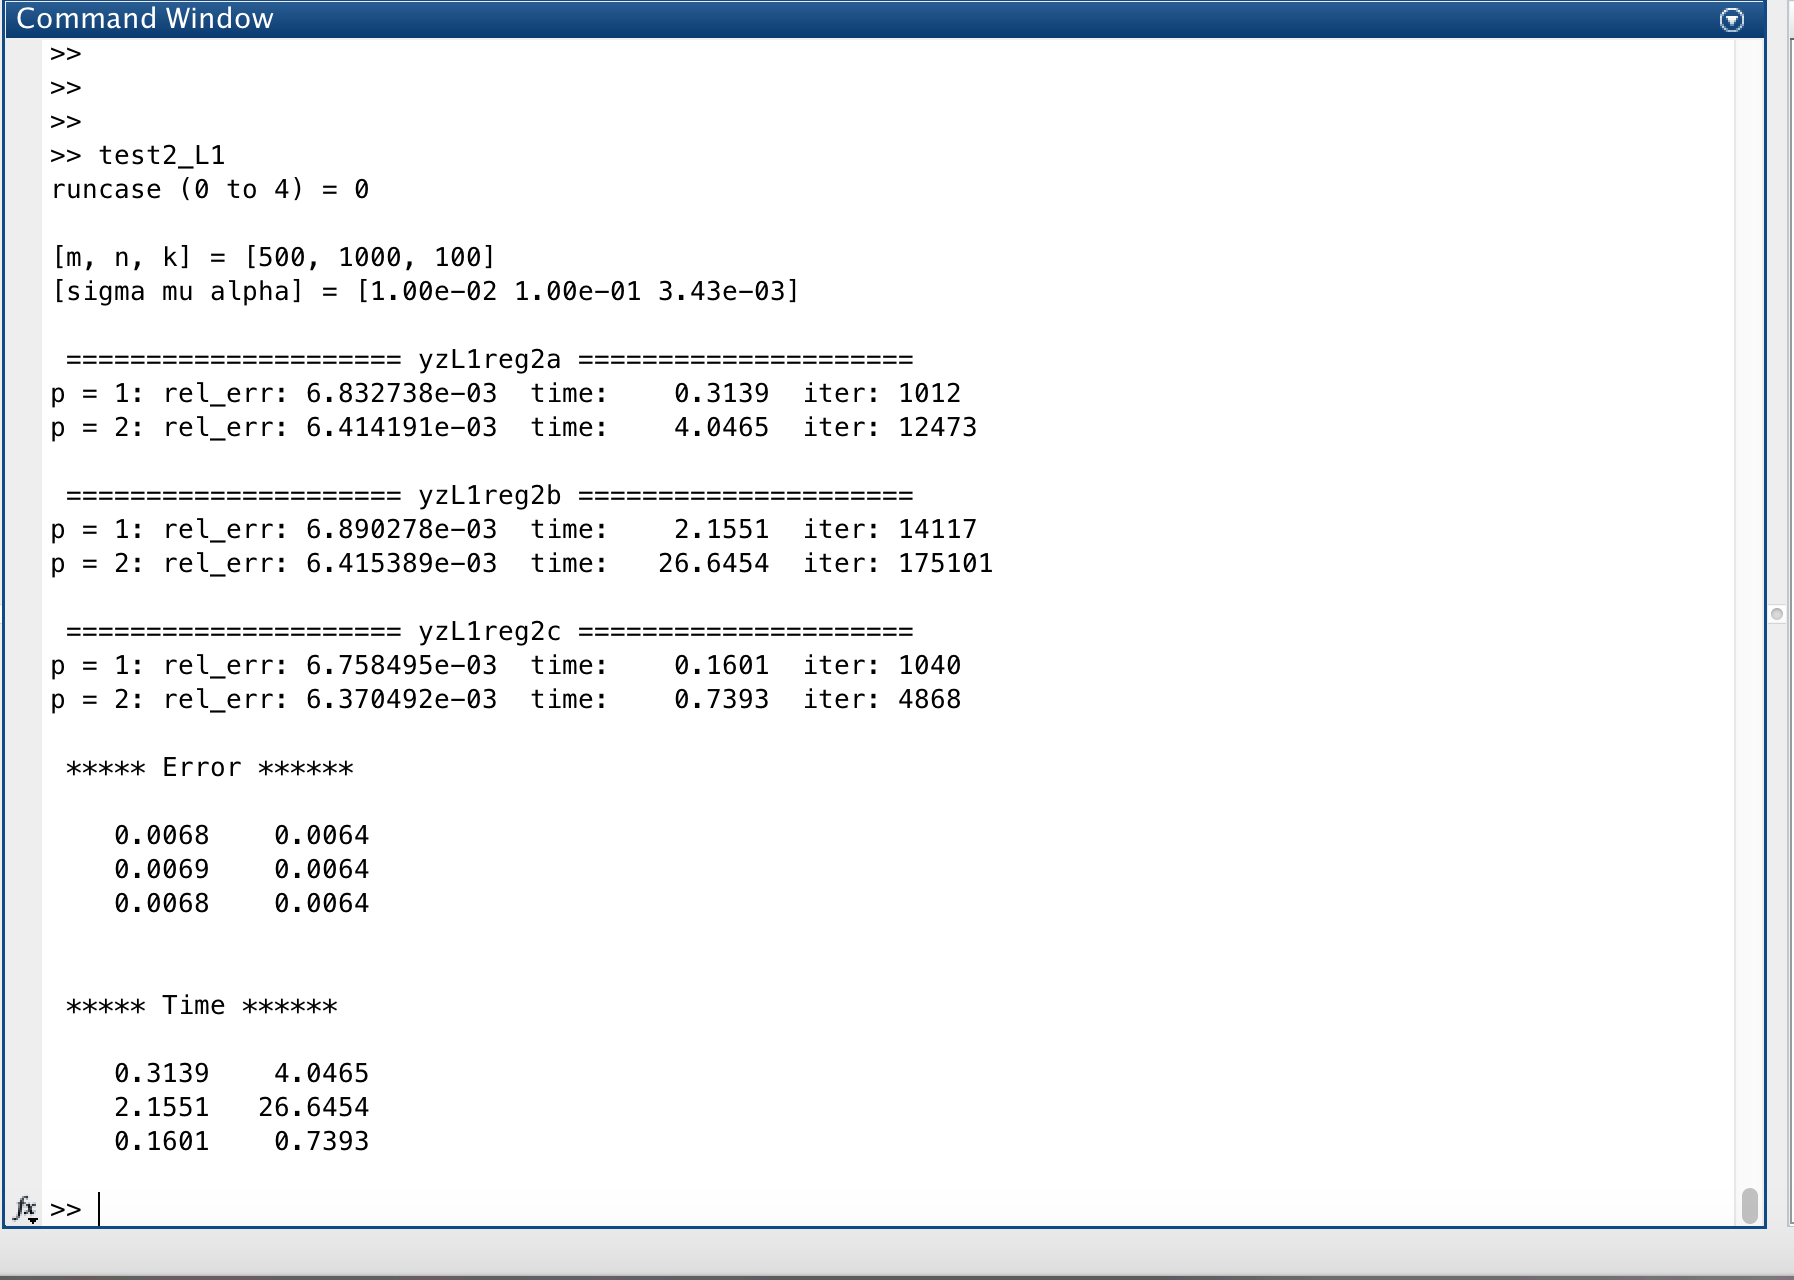
\includegraphics[height=12cm]{p_1}
\caption{Printout from Run Case $1$}
\end{figure}
\begin{figure}[H]
\centering
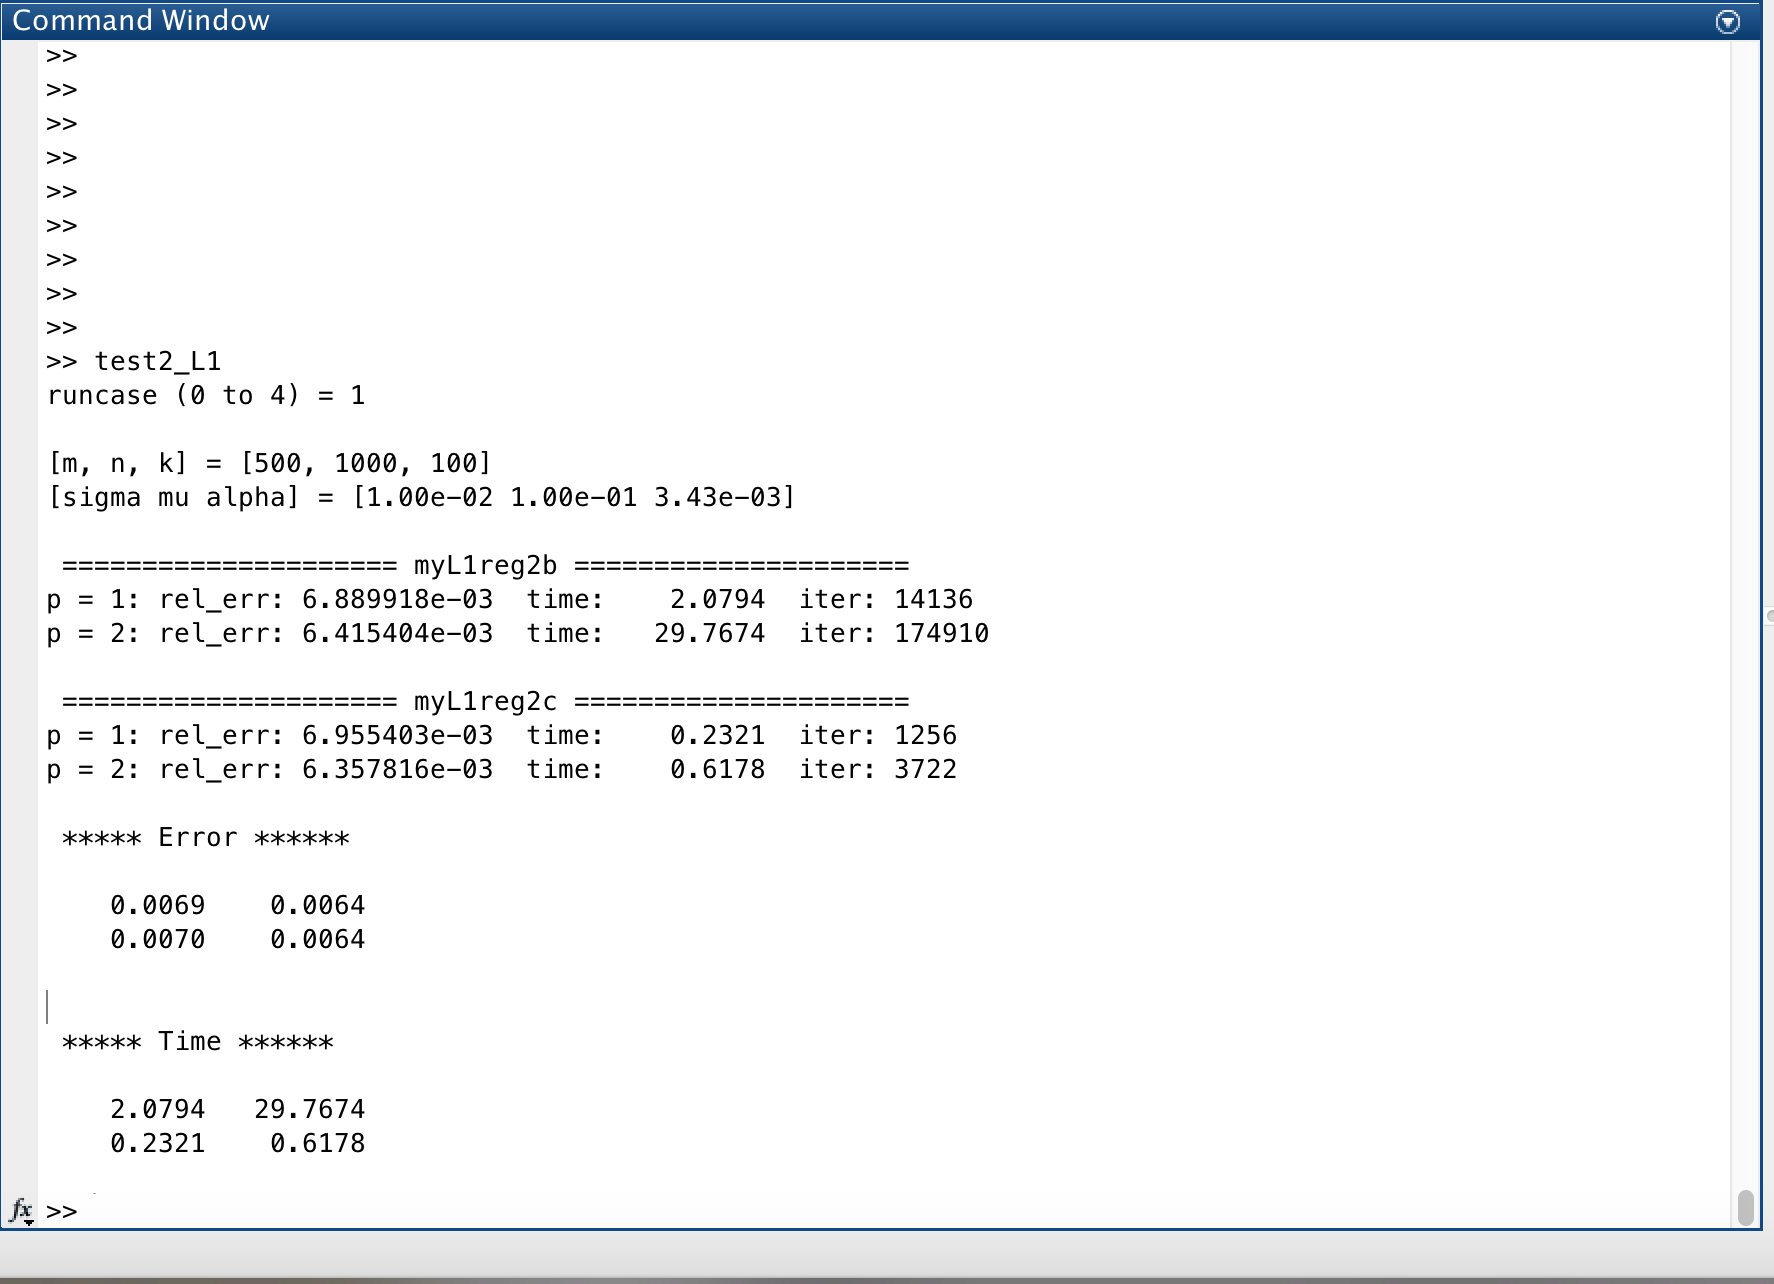
\includegraphics[height=12cm]{p_2}
\caption{Printout from Run Case $2$}
\end{figure}
\begin{figure}[H]
\centering
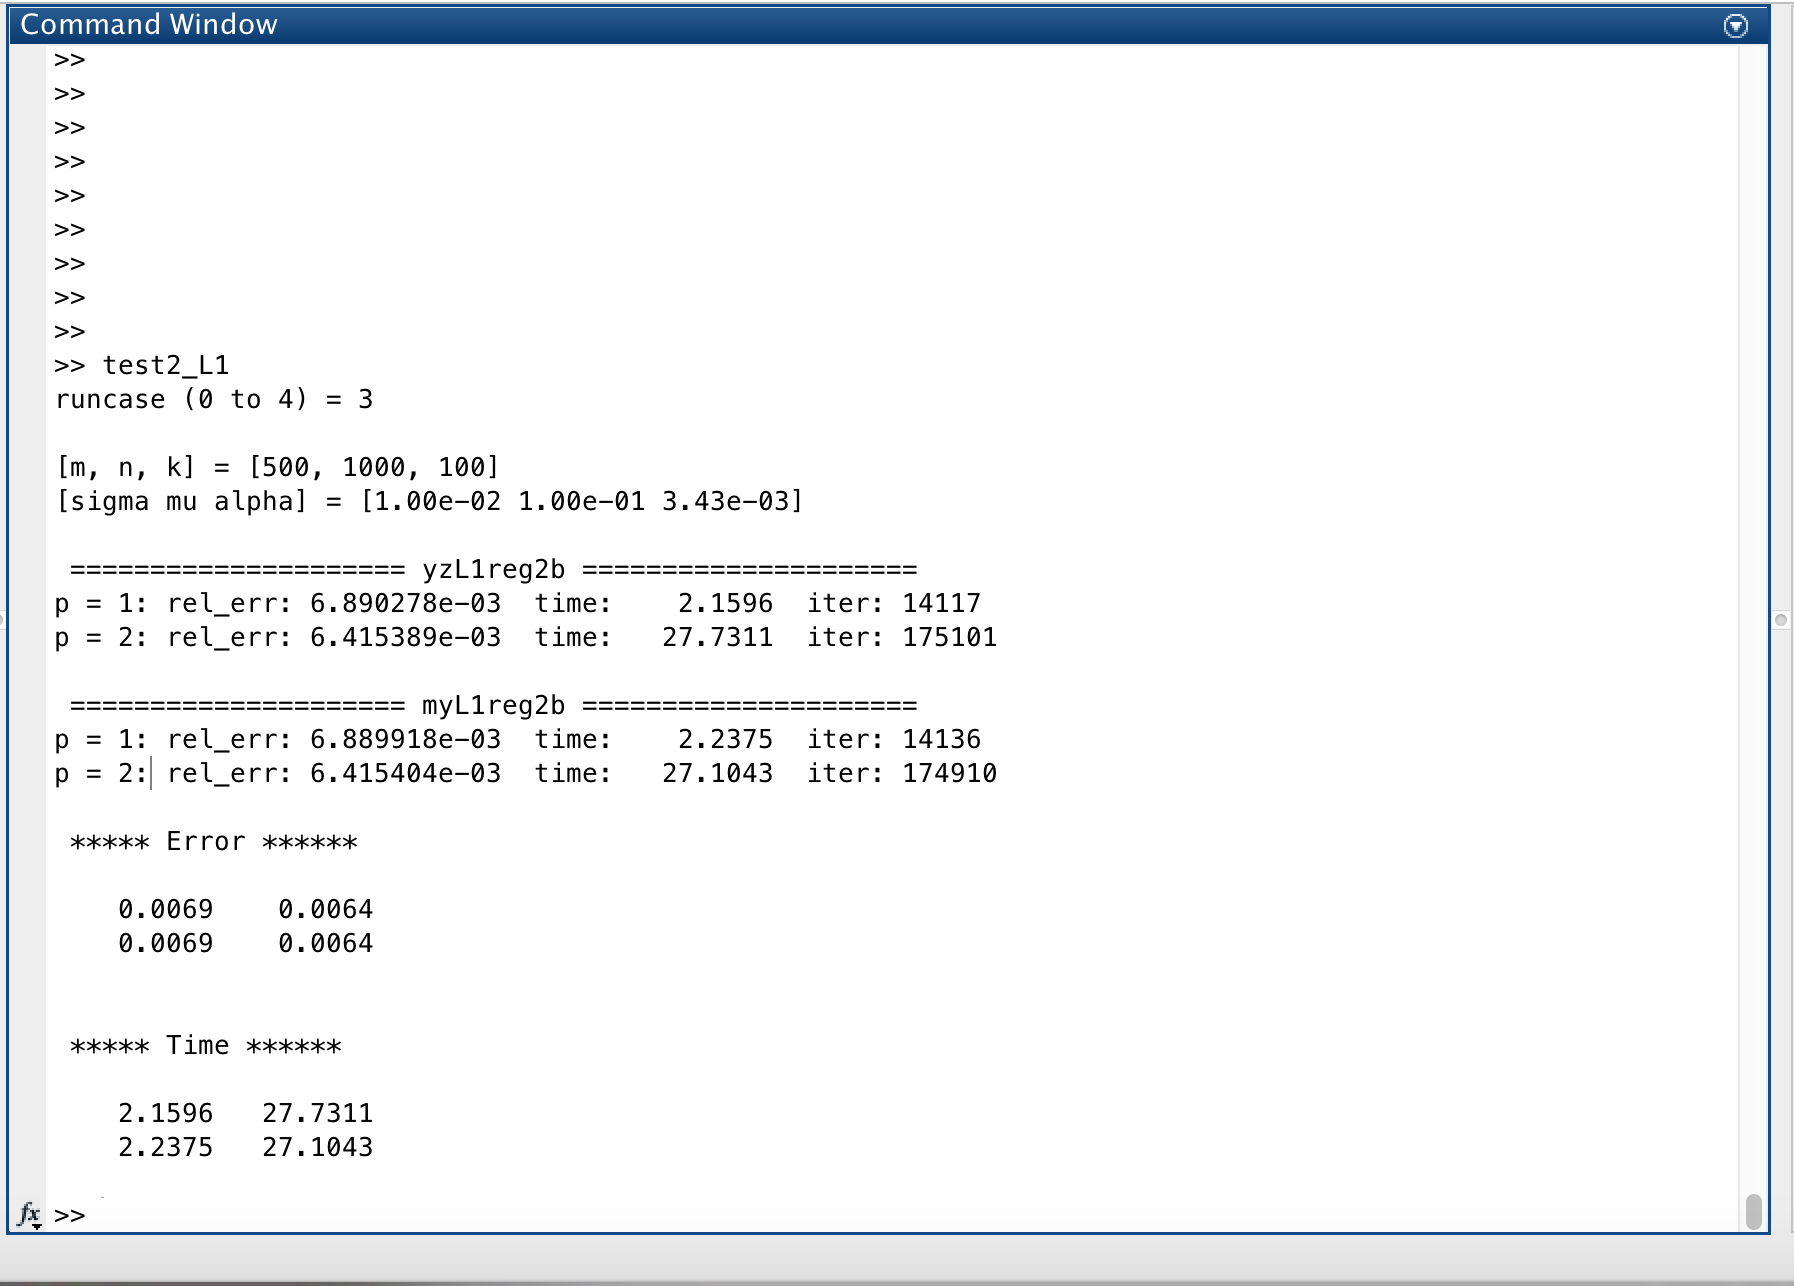
\includegraphics[height=12cm]{p_3}
\caption{Printout from Run Case $3$}
\end{figure}
\begin{figure}[H]
\centering
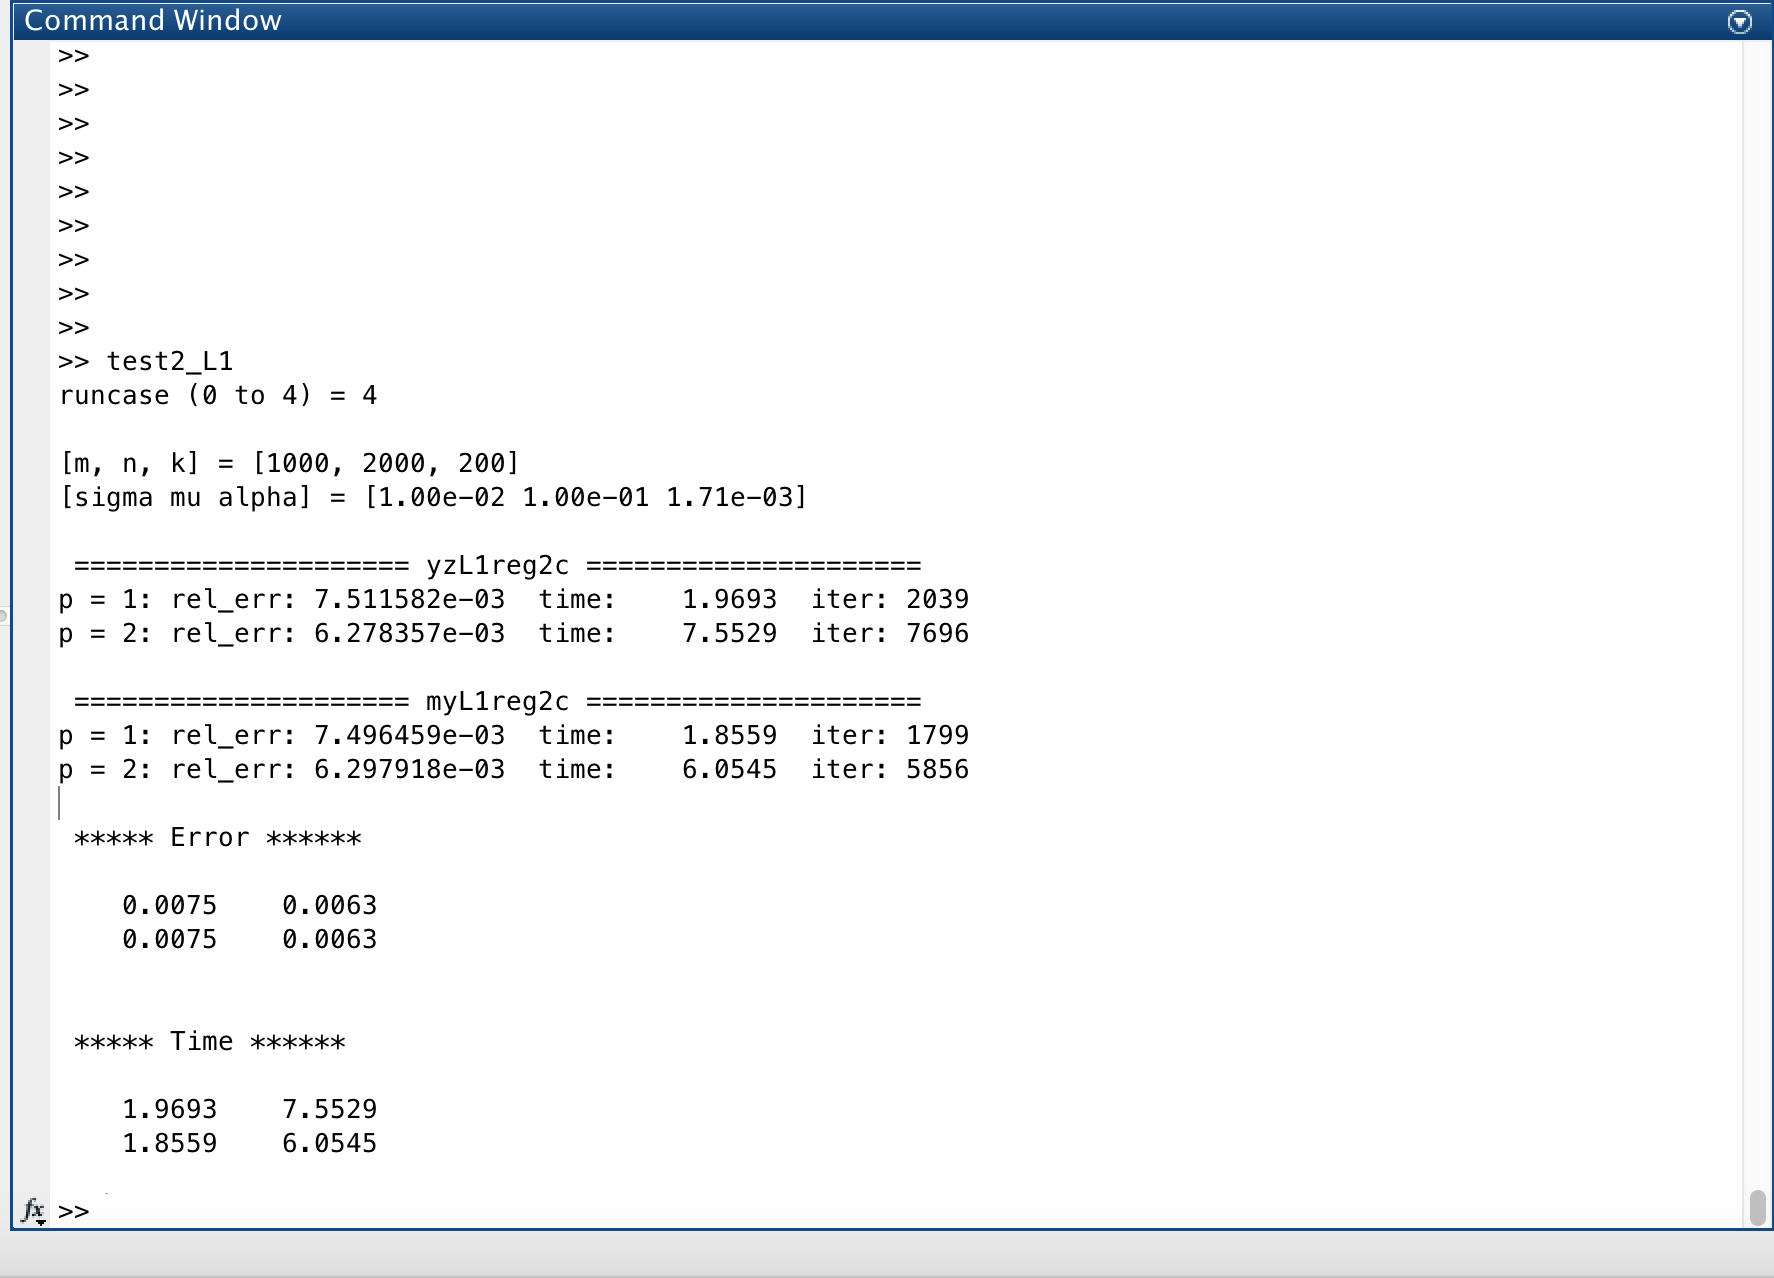
\includegraphics[height=12cm]{p_4.png}
\caption{Printout from Run Case $4$}
\end{figure}

\subsection{Output figure on run case number $4$}
\begin{figure}[H]
\centering
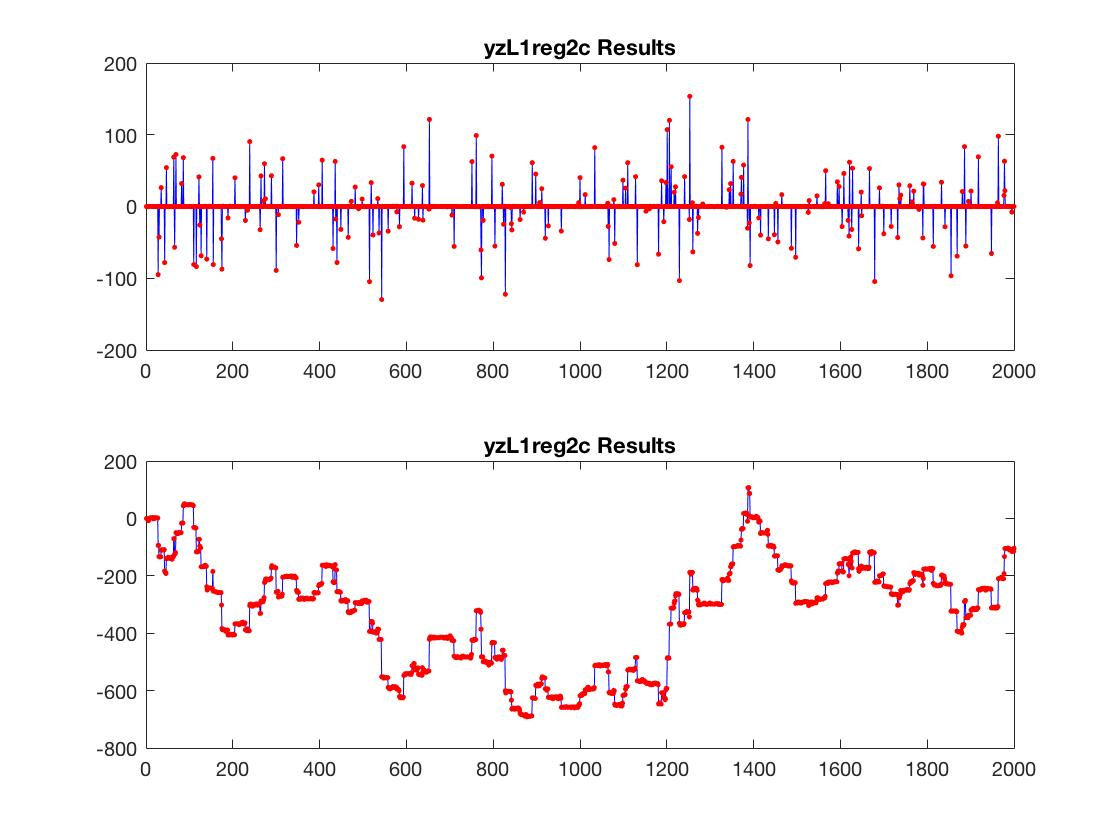
\includegraphics[height=10cm]{p_5}
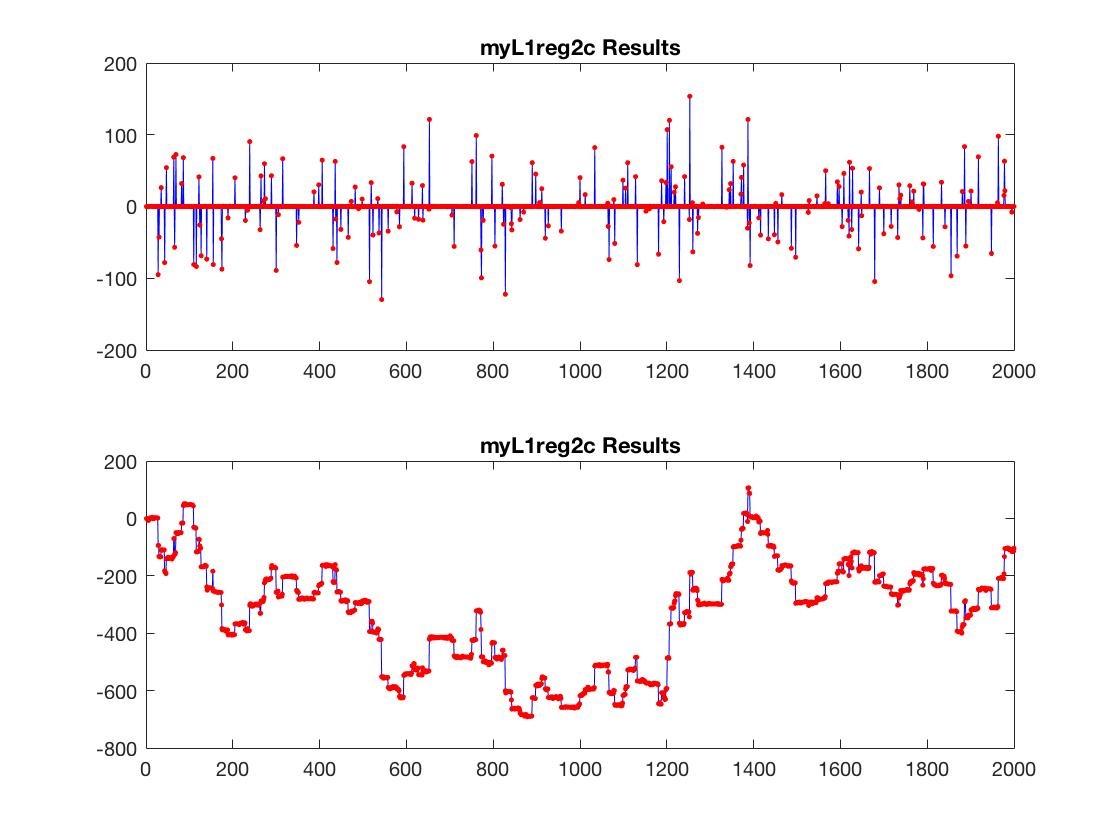
\includegraphics[height=10cm]{p_6}
\caption{Output figure for Run Case $4$}
\end{figure}
\subsection{Short summary about my observations and experiments}
\paragraph{Introduction} This project is about the comparison of three first order methods to solve an unconstrained problem. The first and the second method has different step-size, i.e., the first one is step-size variant while the second is invariant. The third method is optimal among all first order methods, i.e., it will obtain fastest speed in worse case.

\paragraph{Comments about step-size-invariant method}
Although the step-size-invariant method also guarantees the convergence and the error using this method is also very small in this project, it has too small step-size ($\frac{1}{L}$) such that the convergence rate is very small. In large scale optimization, every iteration for computing the gradient is expansive, thus the step-size-invariant method is not recommended in this case as it requires many iterations, i.e., too much computation and time resources.
\paragraph{Comments about step-size variant method}
If applying step-size variant method, there may also rise some problems. First, the choice of step-size may spend lots of time. Second, the step-size variant method only choose $\{\nabla g(x_1),\dots,\nabla g(x_k),\dots\}$ sequentially as the descent direction. In practice, such method may not receive satisfying results as well.
\paragraph{Comments about accelerated method}
The Nesterov’s optimal method is an alternative way to rescue the step-size invariant method, i.e., it has fixed step-size, but for each iteration it also use part of the direction from last iteration. With combination of two diredctions (last and this iteration), this method has faster convergence rate than that with only one direction.






\clearpage
\section{MATLAB Project: Newton’s Method}
\subsection{Three Copies of my Code}
\begin{lstlisting}[language=matlab]
function [x, iter ] = myNewton(func, x0, tol, maxit, varargin )
% Implement Newton's method using analytic Jacobian
%  Input:
%   func: function handle
%     x0: initial guess
%    tol: tolerance
%  maxit: maximum iteration
%   varargin - parameters
% Output:
%      x: optimal solution
%   iter: total number of iterations
%% First Iteration
x = x0;
[g,H] = feval(func, x, varargin{:});
nrmg0 = norm(g);
x = x - H \ g;
fprintf('iter: %3d  nrmg/nrmg0 = %6.2e\n',1,1)
%% Remaining iterations
for iter = 2:maxit
    [g, H] = feval(func, x, varargin{:});   % get gradient g and Hessian H
    fraction = norm(g)/nrmg0;
    fprintf('iter: %3d  nrmg/nrmg0 = %6.2e\n',iter,fraction)
    if fraction <= tol,break;end
    x = x - H \ g;
end

end
\end{lstlisting}
\begin{lstlisting}[language=matlab]
function [ x,iter ] = myFdNewton( func,x0,tol,maxit,varargin )
%  Implement Newton's method using finite difference approximation
%  Input:
%   func: function handle
%     x0: initial guess
%    tol: tolerance
%  maxit: maximum iteration
%   varargin - parameters
% Output:
%      x: optimal solution
%   iter: total number of iterations
%% First Iteration
x = x0;
g = feval(func,x,varargin{:});nrmg0 = norm(g);
fprintf('iter: %3d  nrmg/nrmg0 = %6.2e\n',1,1)
H = feval('myHessian',func,x,g,varargin{:});
x = x - H \ g;
%% Remaining iterations
for iter = 2:maxit
    g = feval(func, x, varargin{:});   % get gradient g and Hessian H
    fraction = norm(g)/nrmg0;
    fprintf('iter: %3d  nrmg/nrmg0 = %6.2e\n',iter,fraction)
    if fraction <= tol,break;end
    H = feval('myHessian',func,x,g,varargin{:});
    x = x - H \ g;
end


end


function H = myHessian(func,x,gx,varargin)
%delta = 1e-9;
m = length(gx); n = length(x);
H = zeros(m,n);
for j = 1:n
    epsilon = 1e-9 *  max(1,max(1,abs(x(j))) * sign(x(j)));
    x(j) = x(j) + epsilon;
    g = feval(func, x, varargin{:});
    x(j) = x(j) - epsilon;
    H(:,j) = (g - gx) / epsilon;
end

end
\end{lstlisting}
\begin{lstlisting}[language=matlab]
function [ g,H,f ] = myQuartic( x,A,u,mu )
% Output:
%      g: gradient, g = (x'*A*x - 1/4*u'*A*u) * A*x + mu * (x - u)
%      H: Hessian, H = (x'*A*x - 1/4*u'*A*u) * A + 2*A*x*x'*A + mu * eye(n)
%      f: function itself, 
%      f = 1/4*(x'*A*x - 1/4*u'*A*u) + mu/2 * ||x - u||_2^2

n = length(x);

Ax = A*x;
quartic = x'*Ax - u'*A*u/4;
y = x - u;

%% Evaluate g
g = quartic * Ax + mu * y;
if nargout < 2;return;end

%% Evaluate H
H = quartic * A + 2 * (Ax * Ax') + mu * speye(n);
if nargout < 3;return;end

%% Evaluate f
f = quartic/4 + mu/2 * (y'*y);

end
\end{lstlisting}
\subsection{MATLAB Screen Printout for the run results of \textrm{test quartic.m}}
\begin{figure}[H]
\centering
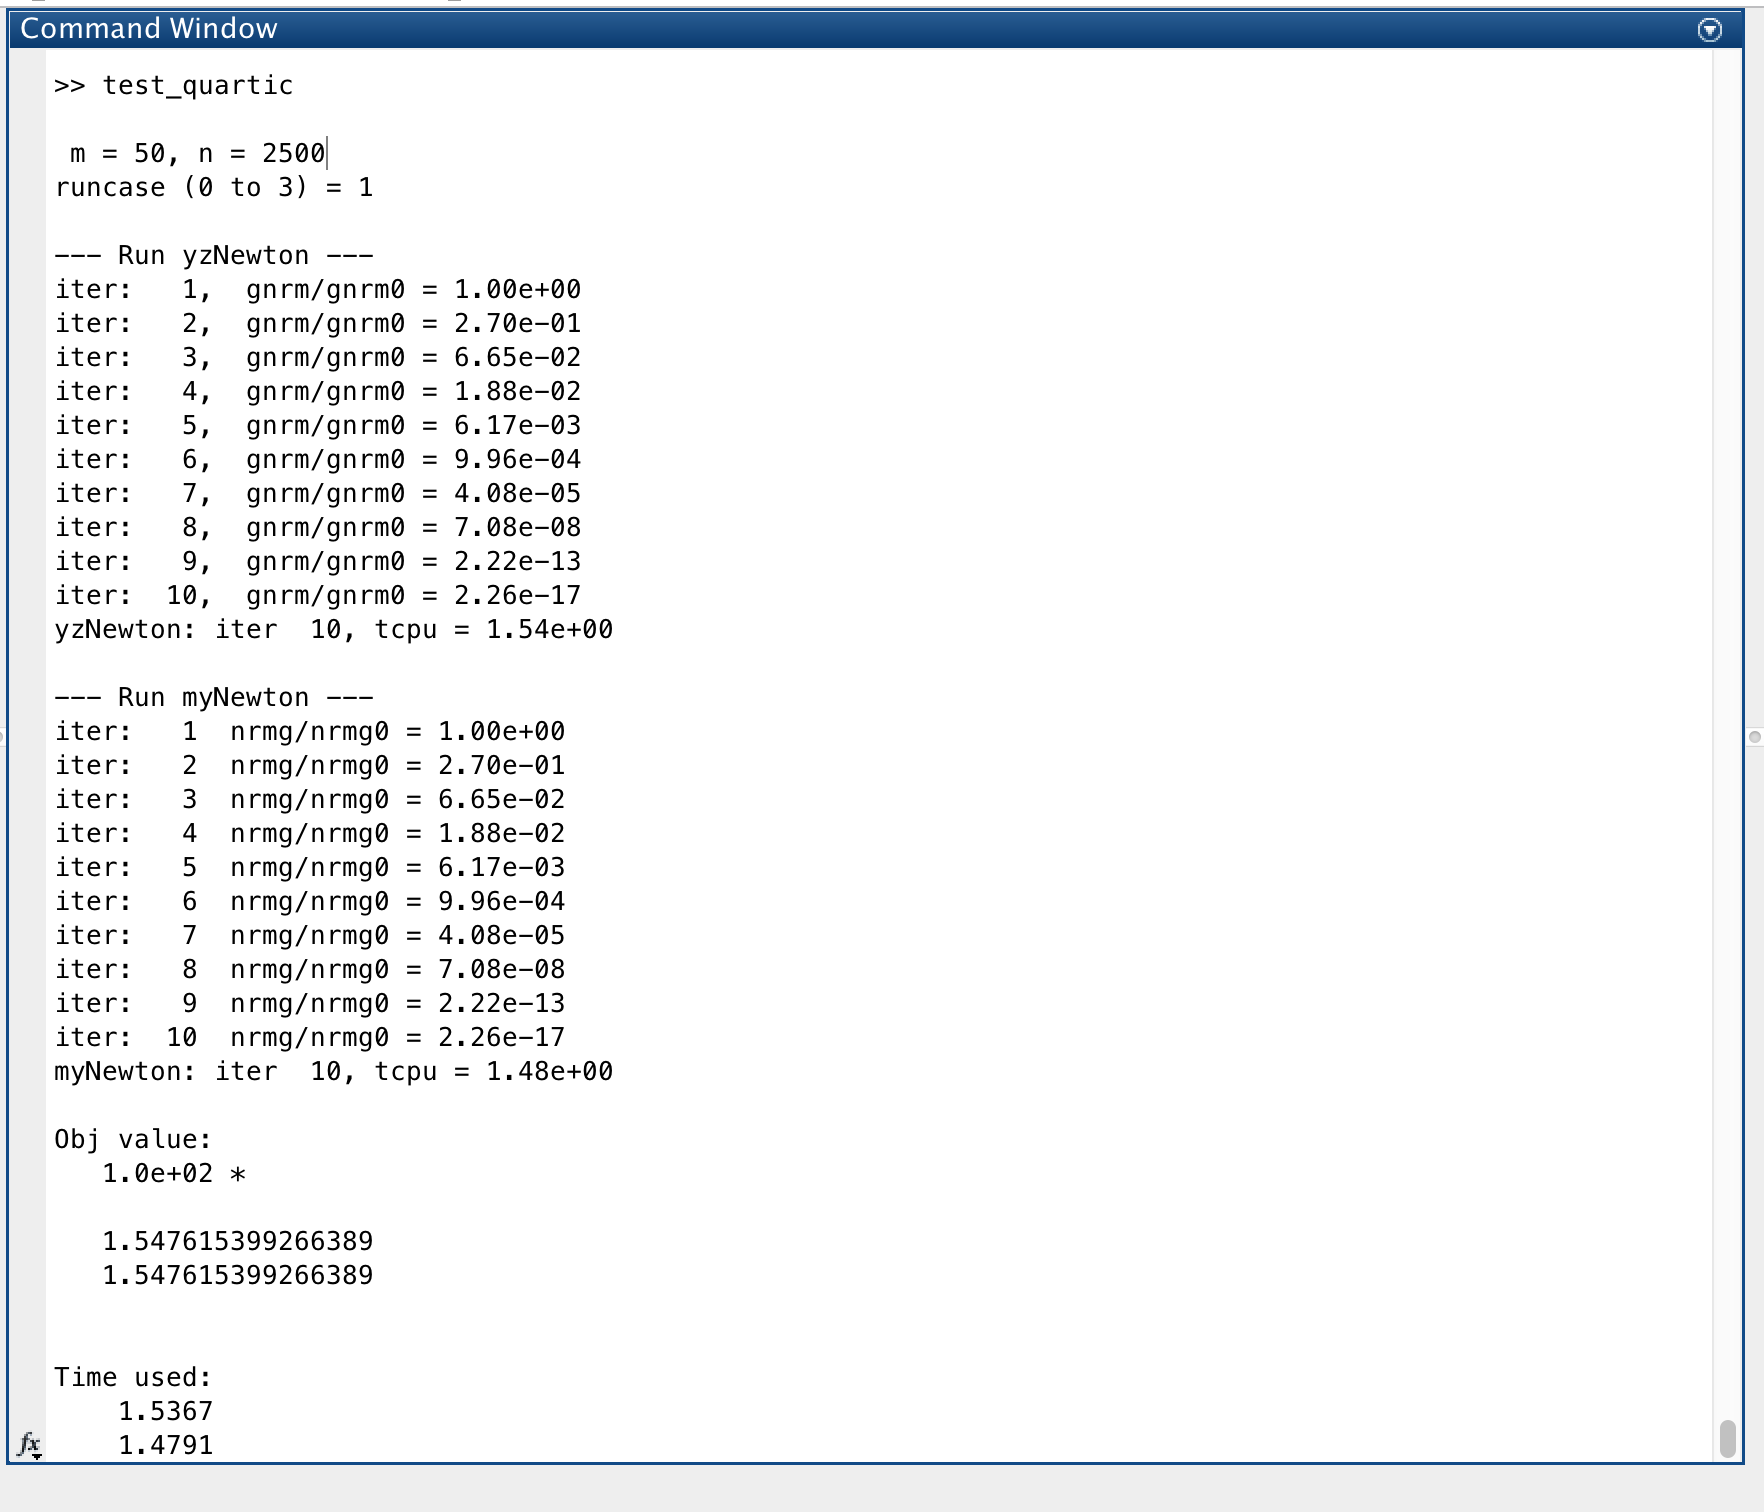
\includegraphics[height=12cm]{p_8}
\caption{Printout from Run Case $1$}
\end{figure}
\begin{figure}[H]
\centering
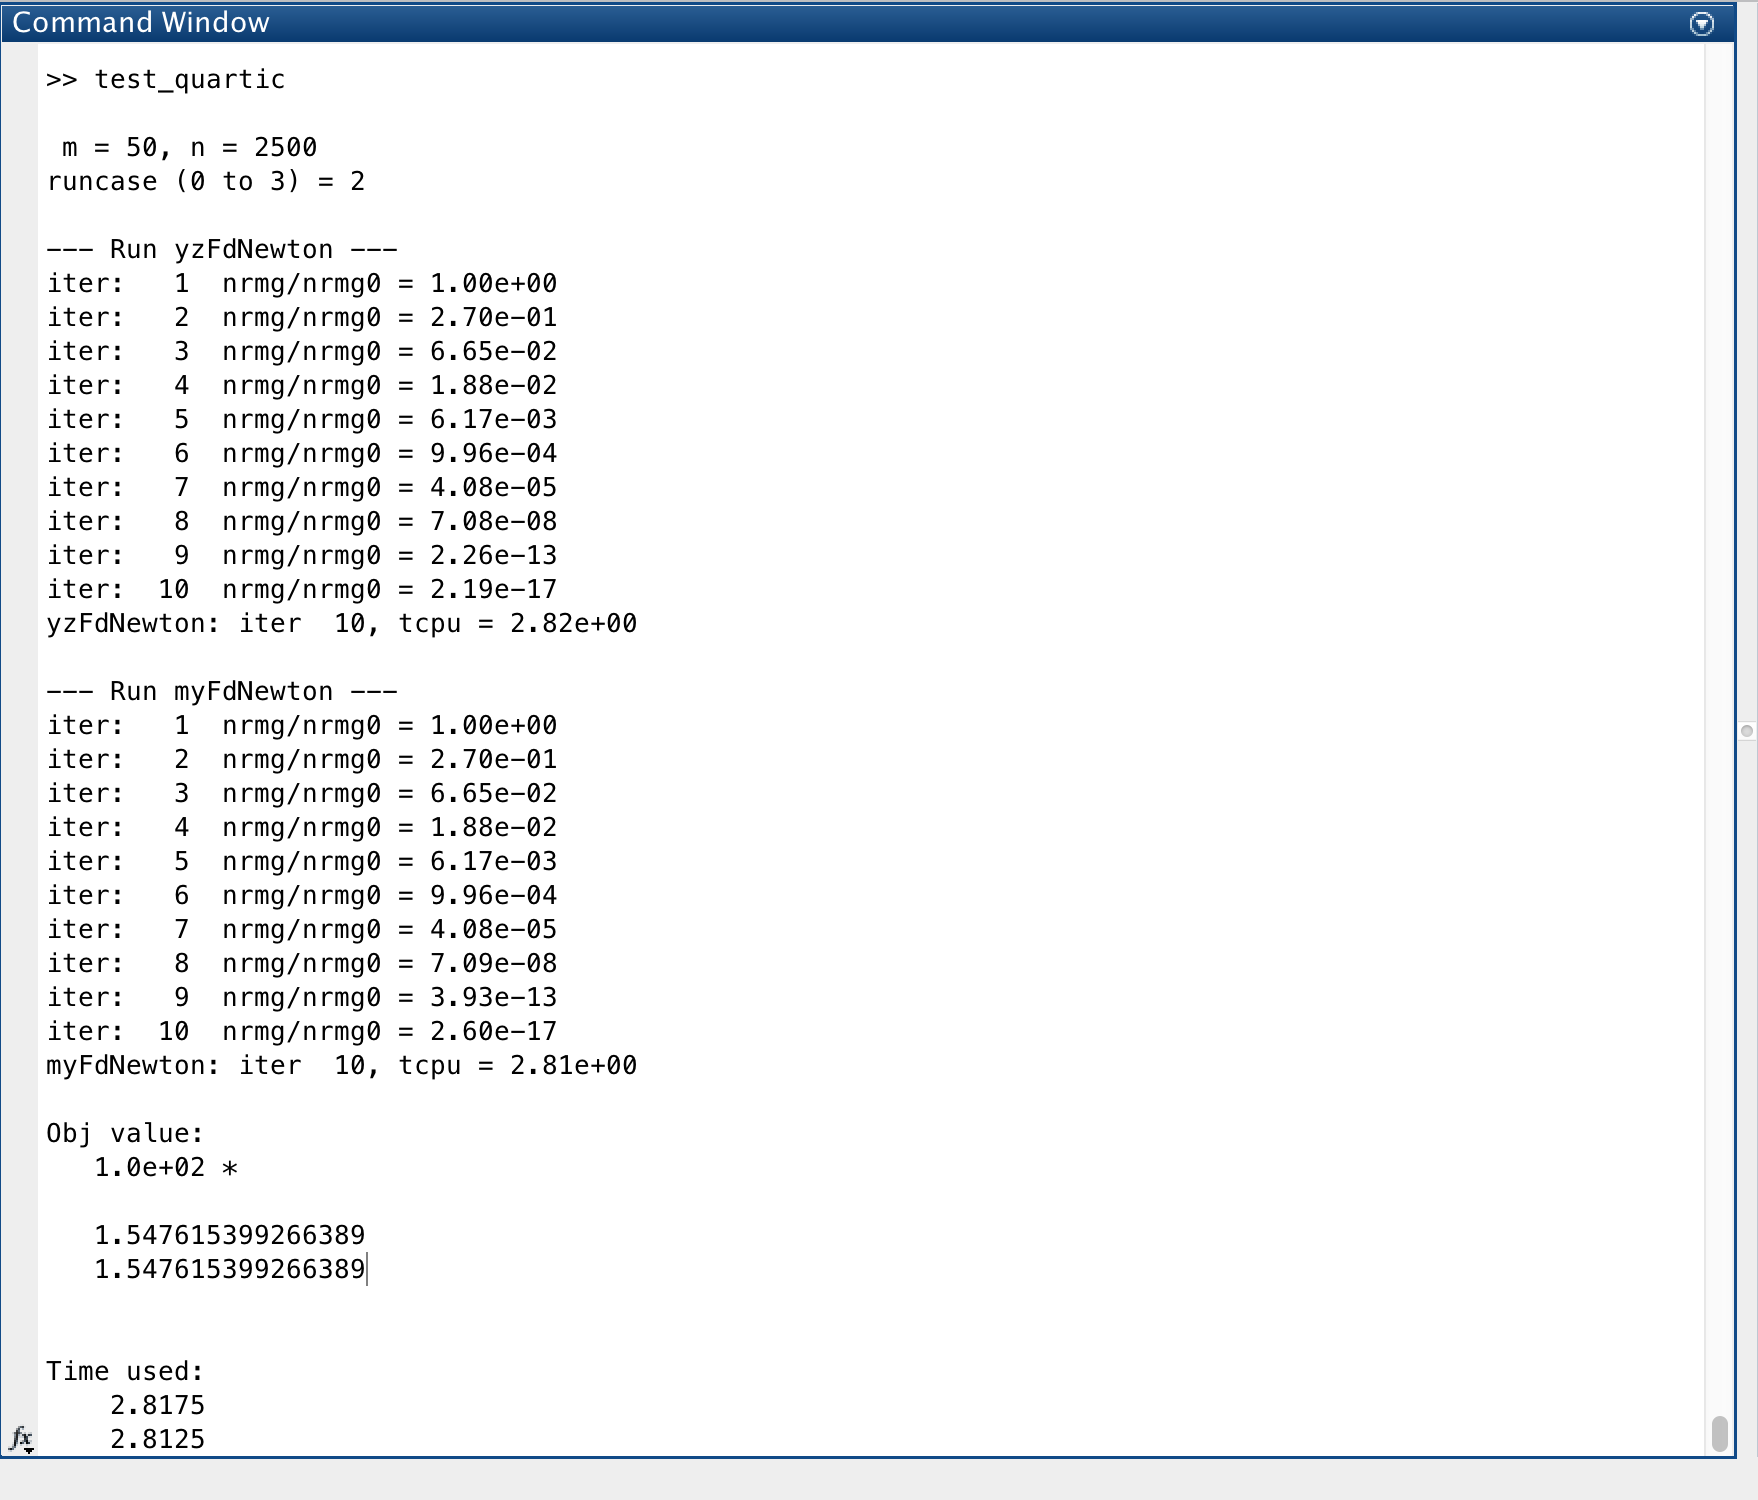
\includegraphics[height=12cm]{p_9}
\caption{Printout from Run Case $2$}
\end{figure}
\begin{figure}[H]
\centering
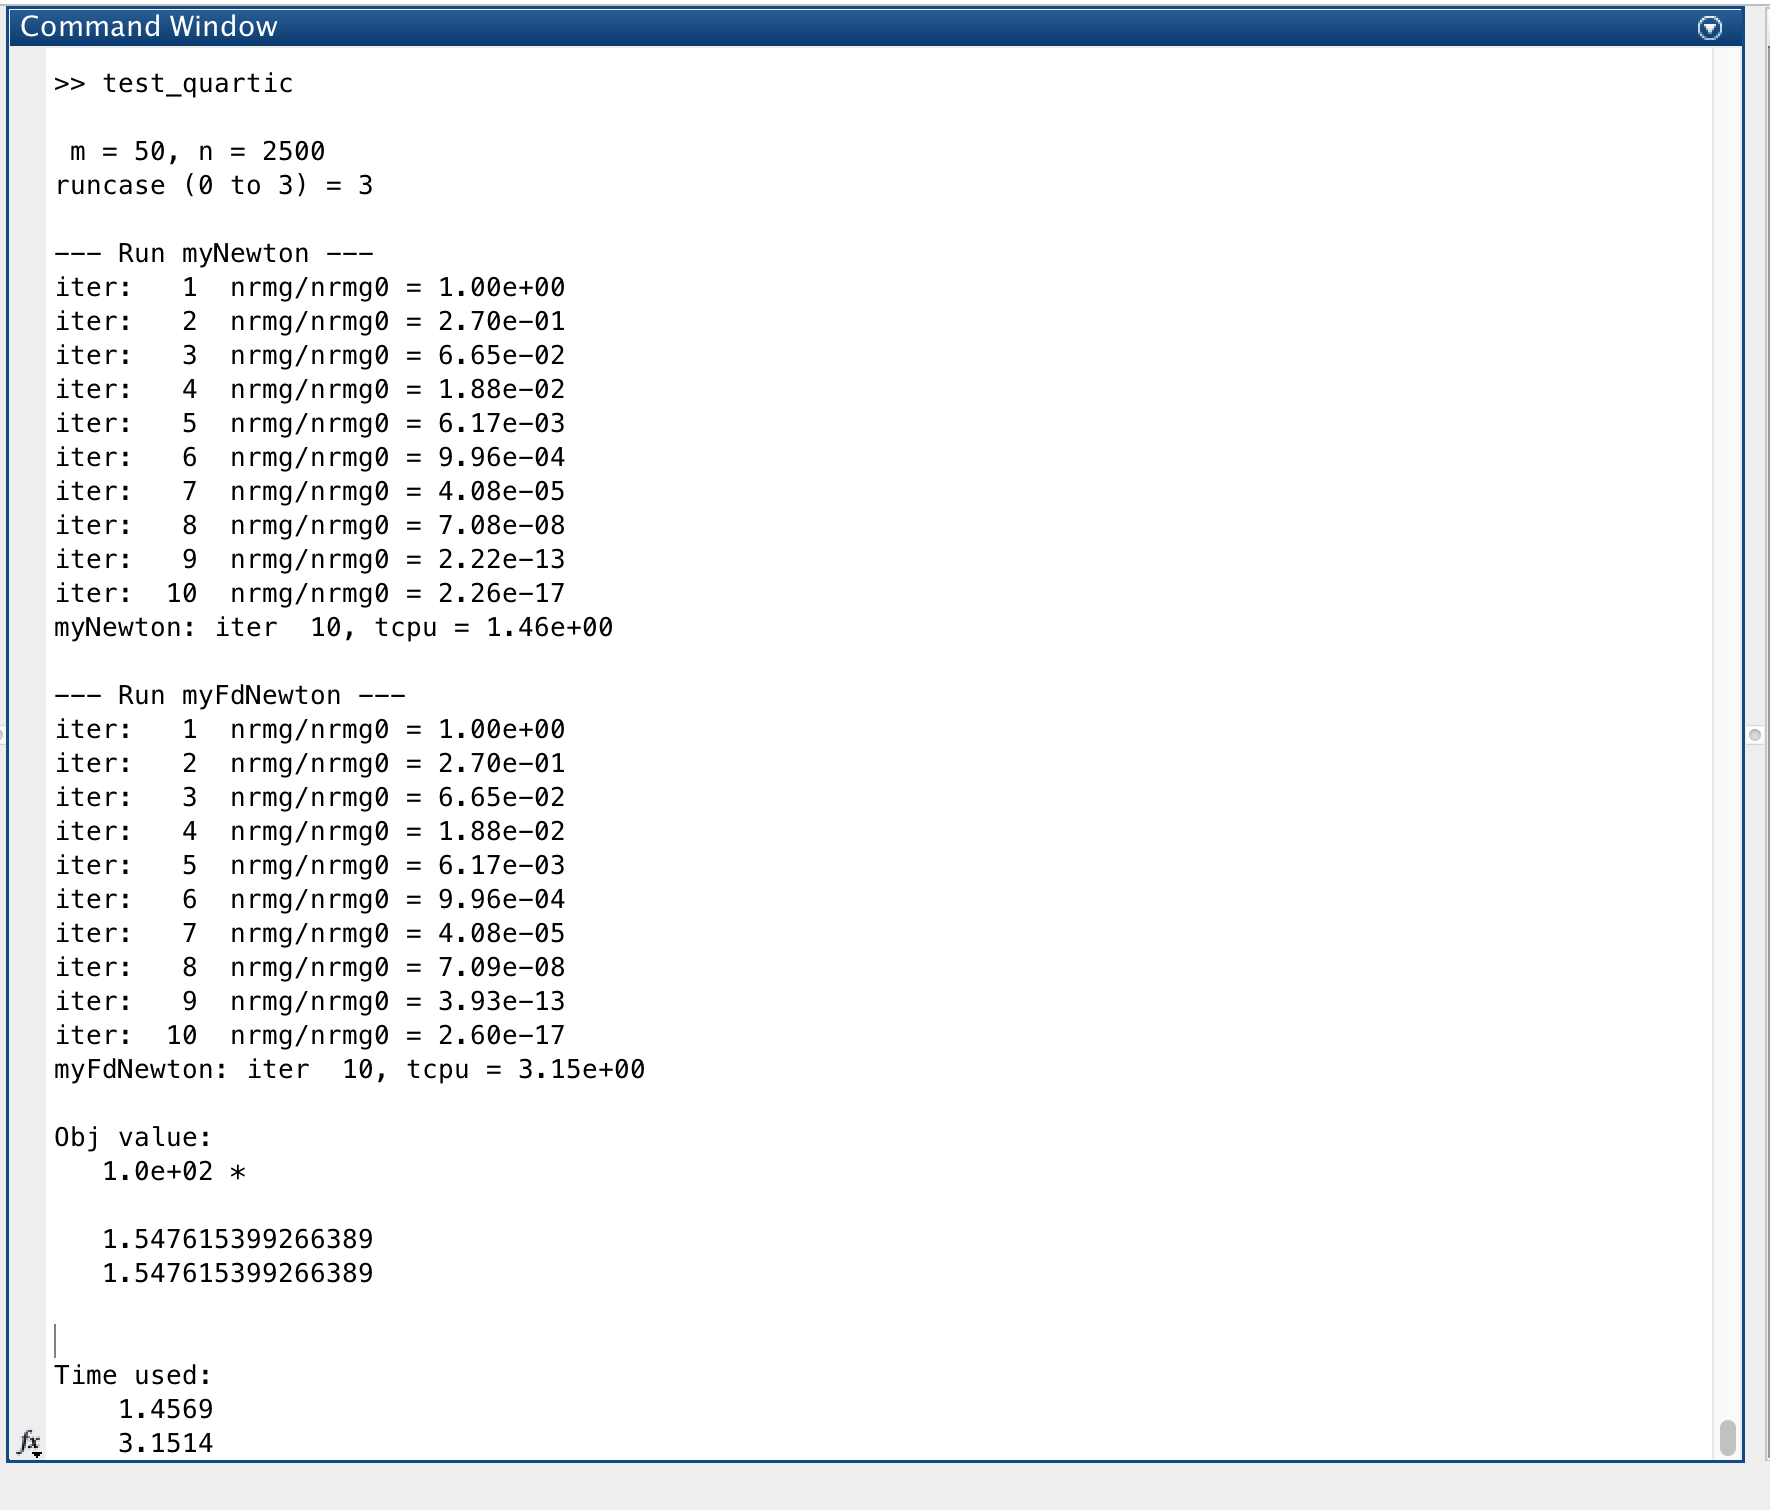
\includegraphics[height=12cm]{p_10}
\caption{Printout from Run Case $3$}
\end{figure}


\subsection{MATLAB Plots generated by \textit{my} codes}
\begin{figure}[H]
\centering
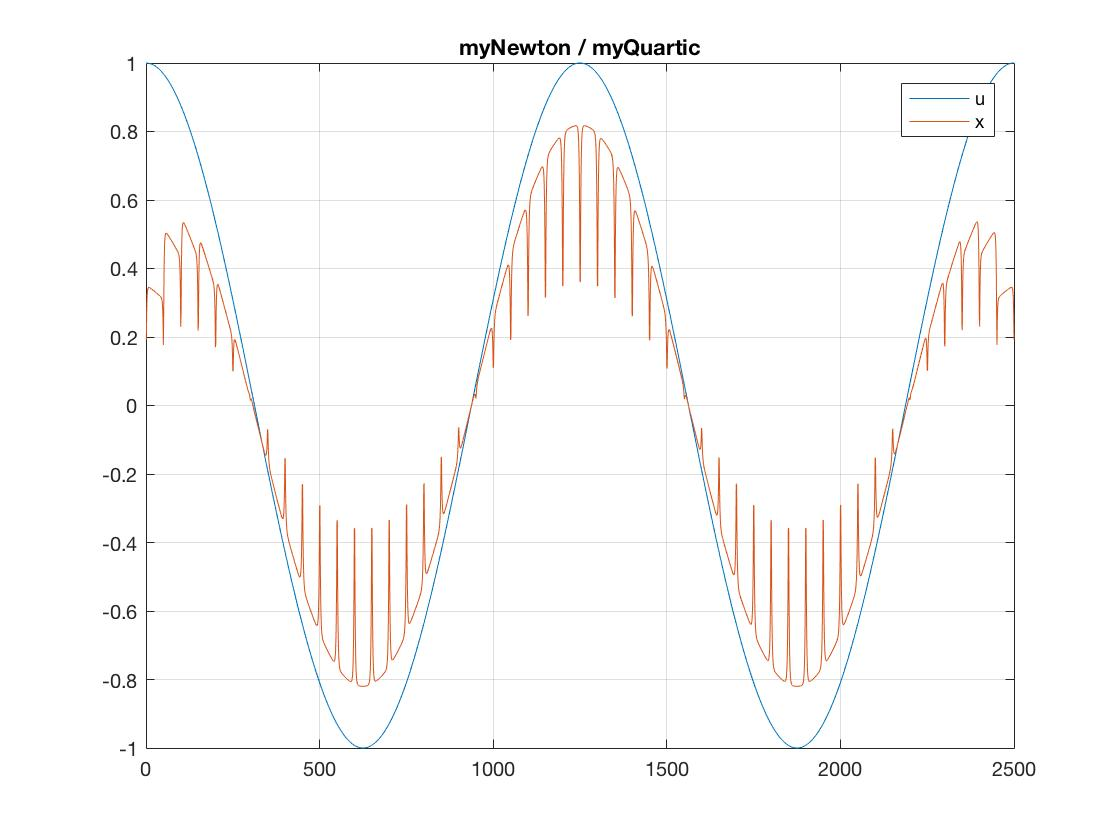
\includegraphics[height=10cm]{p_11}
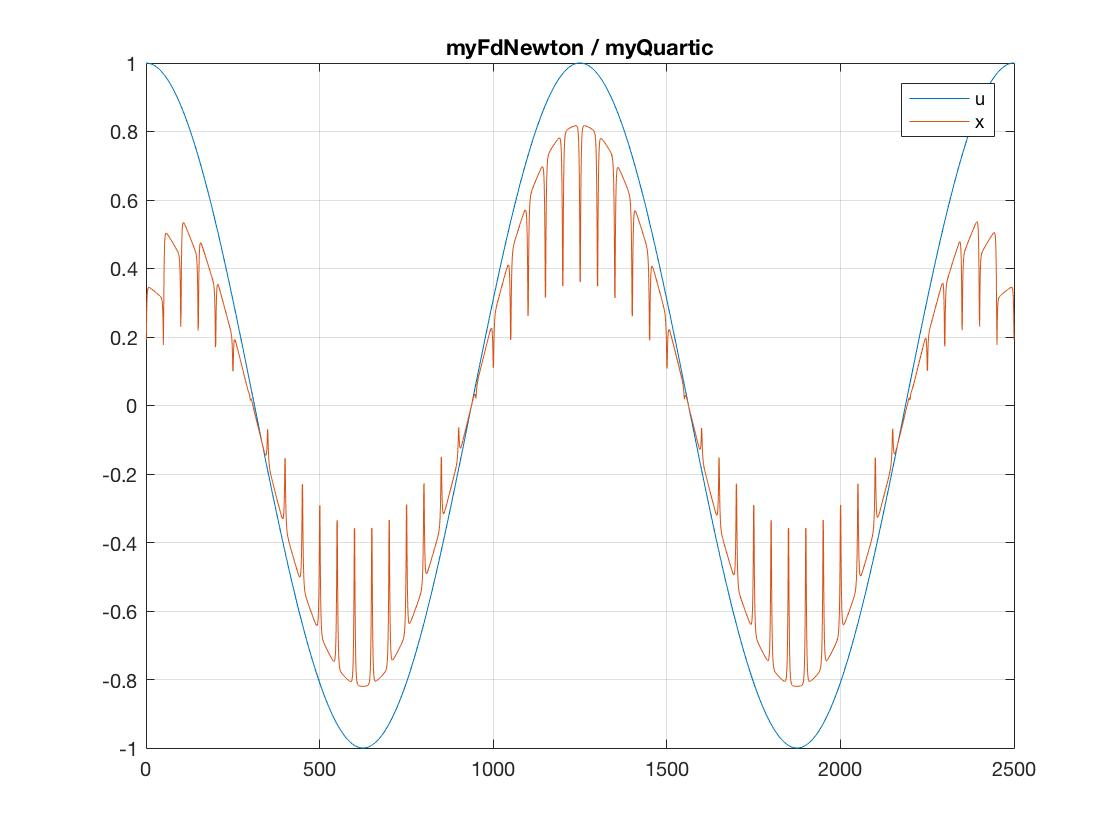
\includegraphics[height=10cm]{p_12}
\caption{MATLAB plots generated by \textit{my} codes (run case = 4)}
\end{figure}

\subsection{Short summary about my experiments and observations}
\paragraph{Introduction}
This project is to solve an unconstrained optimization problem using the pure Newton's methods. The first one computes the Hessian matrix using its analytic form, the second one computes it using finite difference method.
\paragraph{Computation of Hessian matrix is expansive}
We observe that the method using analytic form of Hessian matrix will obtain a faster speed. That's because the numerical approximation of Hessian matrix requires too many iteration, and thus the computation of Hessian matrix in each for loop is very expansive than that of analytic form. 
\paragraph{Comments about the implementation of the quartic function's evaluations}
For the \textrm{myQuartic.m} file, the stop command \textrm{nargout} is necessary, since when calling this funciton, we may not necessarily require the computation of gradient or Hessian matrix, and the computation cost for which is expansive.
\paragraph{Avoid unnecessary computation}
During Newton's method implementation, we should try to avoid the update of function as much as possible, since every update requires the inverse computation of a large dimension matrix. One trick is to put the stop criteria in front of the update command, and therefore the update will stop timely once the stopping criteria is satisfied.
\paragraph{Avoid loss of accuracy during finite difference method}
Two comments about finite difference method to approximate derivative. First, the $h$ for computing $[f(x\pm h)-f(x)]/h$ should have reasonable scale relative to $x$, hence we set $h=10^{-9}\times\max\{1,|x|\}$; second, when $x$ and $h$ have different sign, $x+h$ will loss accuracy due to rounding error in computer. Hence, the approximate of derivative in computer should be modified as $[f(x+ h*\mbox{sign}(x))-f(x)]/h$.
 








\clearpage
\subsection{Derivation and proof for $\mu$ condition}
Since $f$ is continuously differentiable, $f$ is convex iff $\nabla^2f(x)\succeq0$, $\forall x$. We find that:
\begin{align*}
\nabla f(x)&=(x\trans Ax - \frac{1}{4}u\trans Au)*Ax + \mu (x-u)\\
\nabla^2f(x)&=(x\trans Ax - \frac{1}{4}u\trans Au)*A
+Ax*(2x\trans A\trans)+\mu*I\\
&=(x\trans Ax - \frac{1}{4}u\trans Au)*A+2Axx\trans A+\mu*I
\end{align*}
For any $s\in\mathbb{R}^n$, we want to choose $\mu$ such that $s\trans \nabla^2f(x)s\ge0$, or equivalently,
\begin{equation}\label{Eq:1}
(x\trans Ax - \frac{1}{4}u\trans Au)*(s\trans As)
+s\trans Ax*(2x\trans A\trans)s+\mu*s\trans s\ge0,\forall x,\forall s
\end{equation}
We find that $(x\trans Ax)*(s\trans As)+s\trans Ax*(2x\trans A\trans)s\ge0$ for $\forall x$, and choosing $x=0$, $(x\trans Ax)*(s\trans As)+s\trans Ax*(2x\trans A\trans)s=0$, i.e., we obtain the minimum value of LHS of (\ref{Eq:1}):
\begin{align*}
\min_{x}\{(x\trans Ax - \frac{1}{4}u\trans Au)*(s\trans As)
+s\trans Ax*(2x\trans A\trans)s+\mu*s\trans s\}&=-\frac{1}{4}(u\trans Au)*(s\trans As)+\mu*s\trans s\ge0,\forall s
\end{align*}
Or equivalently,
\[
\mu*s\trans s\ge \frac{1}{4}(u\trans Au)*(s\trans As),\forall s\implies
\mu\ge\frac{1}{4}(u\trans Au)*(\frac{s\trans}{\|s\|}A\frac{s}{\|s\|})\forall s
\]
Note that $\max_{s}(\frac{s\trans}{\|s\|}A\frac{s}{\|s\|})=\lambda_{\max}(A)$, which follows that
\[
\mu\ge\max_{s}\frac{1}{4}(u\trans Au)*(\frac{s\trans}{\|s\|}A\frac{s}{\|s\|})=\frac{\lambda_{\max}(A)}{4}(u\trans Au),
\]
i.e., $\mu\ge \frac{\lambda_{\max}(A)}{4}(u\trans Au)$ guarantees convexity of $f(x)$.








\end{document}